% !TEX program = lualatex
\documentclass[11pt,twoside]{article}
\usepackage{apuntes-oscuro}

\asignatura{Ecuaciones Diferenciales}
\cabecera{Tema 4\ \ ·\ \ Guía: variación de las constantes}
\hypersetup{pdftitle={Tema 4. Guía de variación de las constantes},pdfauthor={Daniel Martín Guerrero}}

% ---------- notación (la de las partes I y II) ----------
\newcommand\Lop{\mathcal L}
\newcommand\yh{\hat y}
\newcommand\vyh{\hat{\bm y}}
\newcommand\vk{\bm k}
\newcommand\vb{\bm b}
\newcommand\ve{\bm e}
\newcommand\abs[1]{\lvert#1\rvert}
\newcommand\mat[1]{\begin{pmatrix}#1\end{pmatrix}}
\newcommand\smat[1]{\left(\begin{smallmatrix}#1\end{smallmatrix}\right)}
\newcommand\pI[1]{(P1,~#1)}
\newcommand\pII[1]{(P2,~#1)}
\providecommand\senh{\operatorname{senh}}

\begin{document}

% =====================================================================
%  PORTADA
% =====================================================================
\begin{titlepage}
\thispagestyle{empty}
\centering
\vspace*{-0.6cm}

\includegraphics[width=4.6cm]{figuras/usal.png}\par
\vspace{0.75cm}
{\color{sky}\rule{\textwidth}{0.5pt}}\par
\vspace{0.55cm}
{\color{muted}\small\textls[220]{\textsc{Facultad de Ciencias}}\quad·\quad\textls[220]{\textsc{Grado en Física}}}\par
\vspace{1.25cm}
{\color{acc}\textls[260]{\textsc{Ecuaciones Diferenciales}}}\par
\vspace{0.2cm}
{\color{muted}\small\textls[260]{\textsc{Tema 4\ \ ·\ \ Guía de ejercicios}}}\par
\vspace{1.25cm}
{\fontsize{27}{33}\selectfont\bfseries Variación de las constantes\par}
\vspace{0.12cm}
{\fontsize{19}{24}\selectfont\bfseries método, atajos y ejercicios resueltos\par}
\vspace{0.55cm}
{\color{acc}\rule{2.4cm}{0.8pt}}\par
\vspace{0.45cm}
{\color{muted}\small\itshape Forma normal\quad·\quad Wronskiano y regla de Cramer\quad·\quad Núcleo de Green\par
Reducción de orden\quad·\quad Seminario resuelto\quad·\quad Ejercicios propuestos\par}
\vspace{0.45cm}
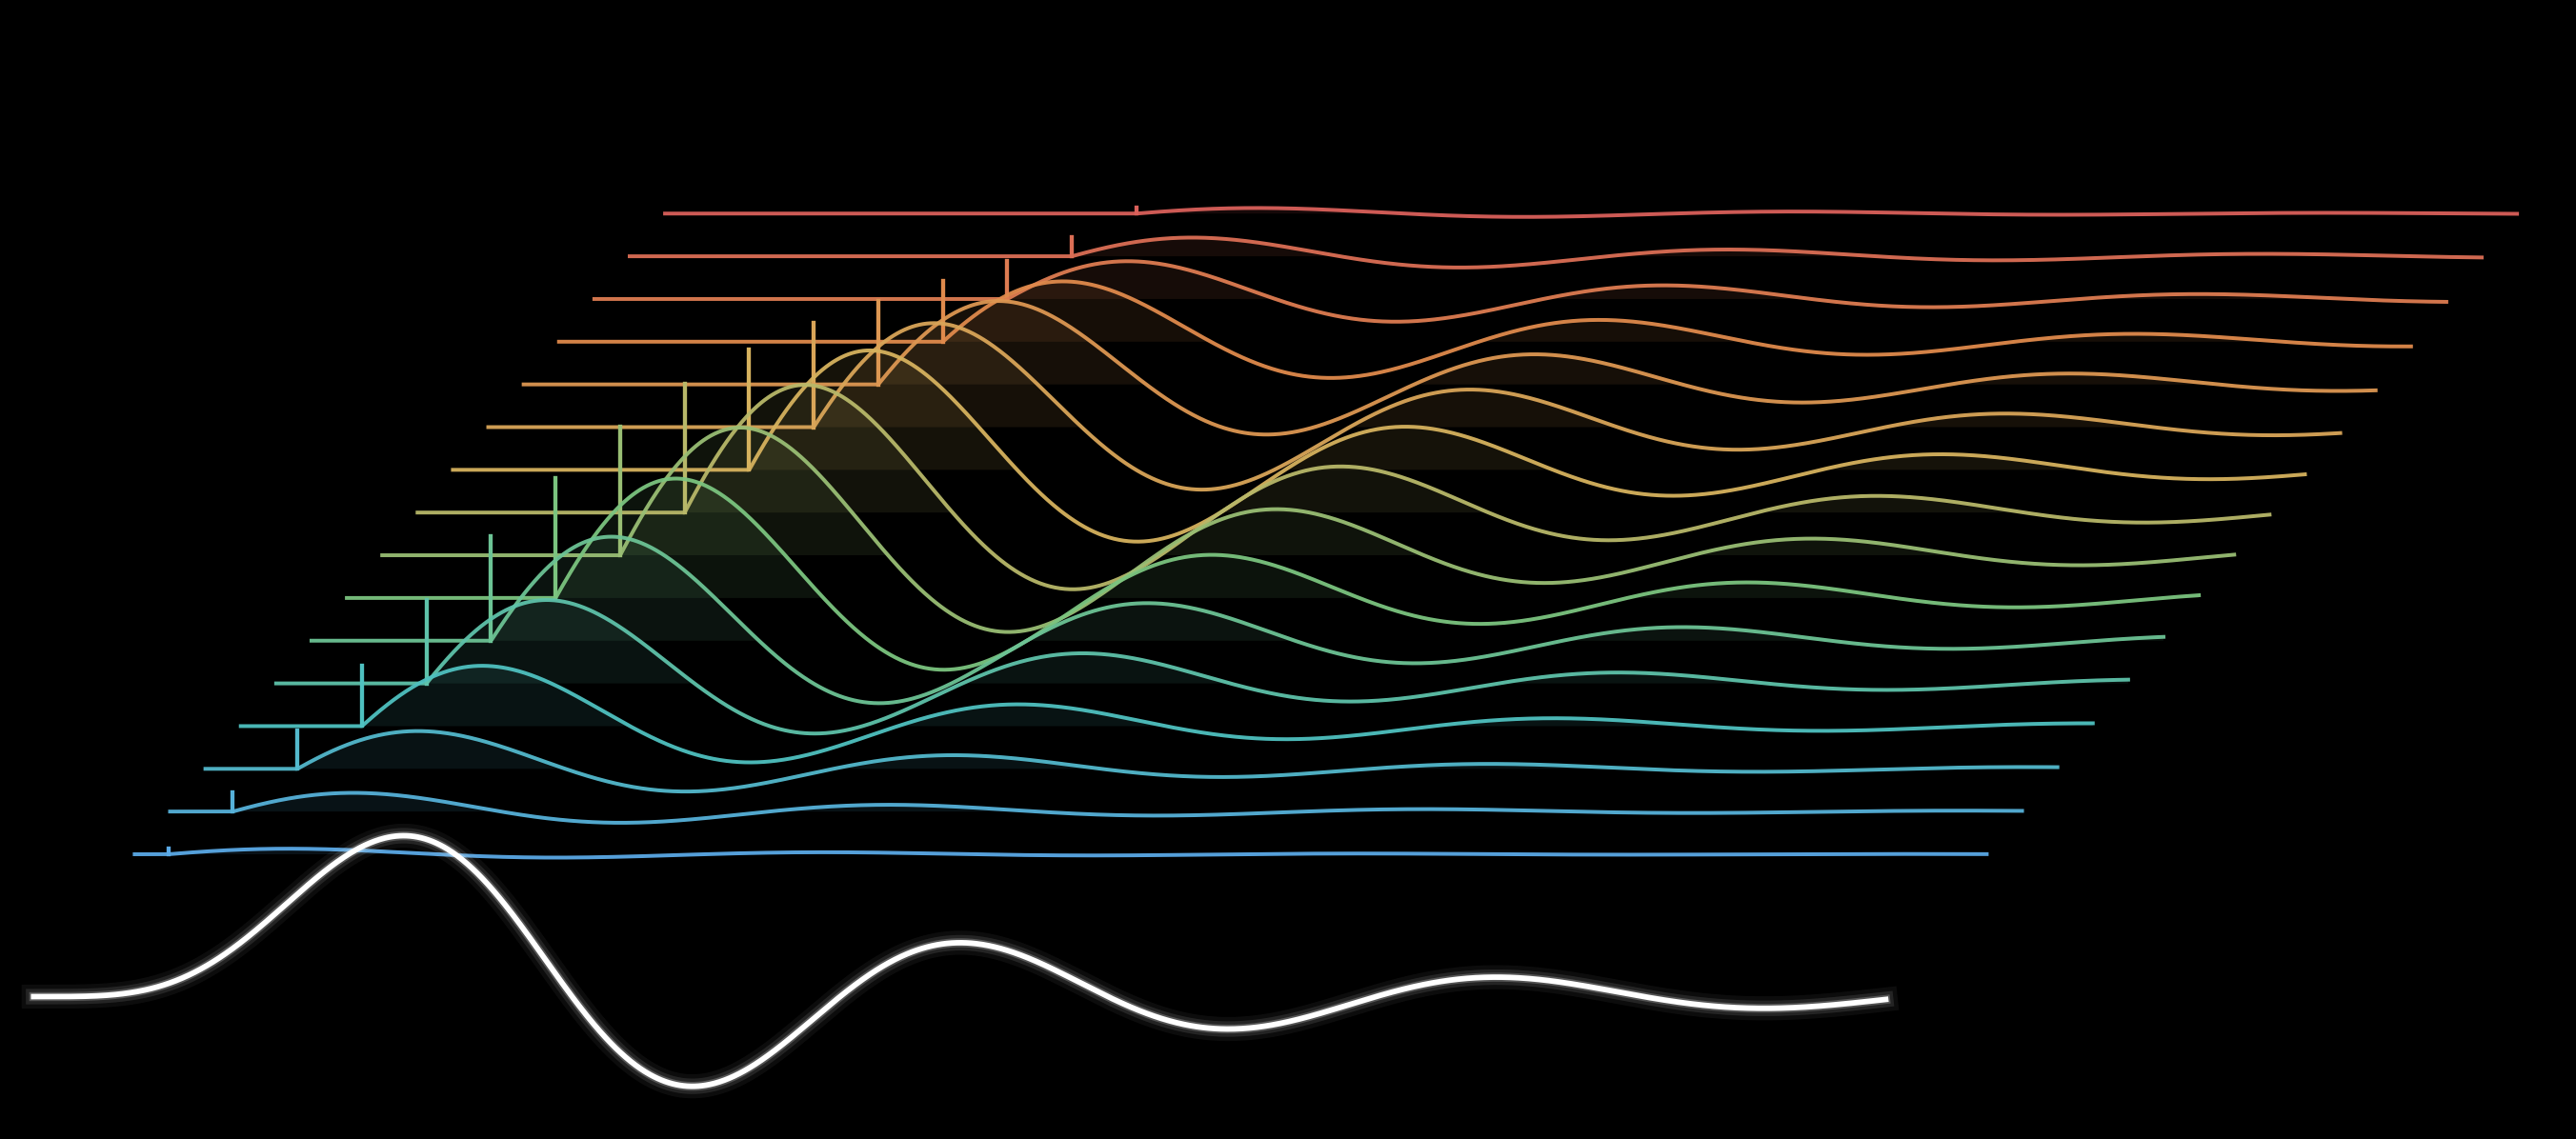
\includegraphics[width=0.86\textwidth]{figuras/portada_t4p1.png}\par
\vspace{0.35cm}
{\small$\displaystyle W\,\vk'=\frac{b}{a_n}\,\ve_n\quad\Longrightarrow\quad
y_p(x)=\vyh\T(x)\int_{x_0}^{x}W^{-1}(s)\,\ve_n\,\frac{b(s)}{a_n(s)}\,\dd s$\par}
\vfill
{\color{sky}\rule{\textwidth}{0.5pt}}\par
\vspace{0.3cm}
\begin{minipage}[t]{0.32\textwidth}\raggedright
{\color{acc}\footnotesize\textls[200]{\textsc{Autor}}}\par\vspace{2pt}
{\small Daniel Martín Guerrero}
\end{minipage}\hfill
\begin{minipage}[t]{0.32\textwidth}\centering
{\color{acc}\footnotesize\textls[200]{\textsc{Profesorado}}}\par\vspace{2pt}
{\small Pilar García Estévez\\ José Beltrán Jiménez\\ María Pérez Garrote}
\end{minipage}\hfill
\begin{minipage}[t]{0.32\textwidth}\raggedleft
{\color{acc}\footnotesize\textls[200]{\textsc{Apuntes formalizados}}}\par\vspace{2pt}
{\small Salamanca, curso 2026/2027}\\[1pt]
{\footnotesize\color{muted}Guía práctica y seminario}
\end{minipage}
\end{titlepage}

\setcounter{page}{2}
{\hypersetup{linkcolor=fg}\tableofcontents}
\clearpage

% =====================================================================
\section{La idea en una página}\label{sec:idea}
% =====================================================================

\begin{motivacion}{Para qué sirve esta guía}
La variación de las constantes es el método \emph{universal} para la solución particular de una EDO lineal: no pide
coeficientes constantes ni una fuente «bonita», sólo una base de la homogénea. Aquí lo reducimos a una receta
(sección~\ref{sec:metodo}), damos los atajos que ahorran cuentas (sección~\ref{sec:atajos}) y lo aplicamos a los ejemplos
de clase y a todos los problemas del seminario donde aparece (secciones~\ref{sec:ejemplos} y~\ref{sec:seminario}). Al
final hay ejercicios propuestos con solución (sección~\ref{sec:propuestos}). Citamos la parte I como (P1, \dots) y la
parte II como (P2, \dots).
\end{motivacion}

Partimos de $\Lop[y]=a_n(x)\,y^{(n)}+\dots+a_0(x)\,y=b(x)$ con $a_n\neq0$ en el intervalo $I$, y de una base
$\yh_1,\dots,\yh_n$ de $\ker\Lop$. La idea es \emph{promover las constantes a funciones}:
\begin{equation}\label{eq:ansatz}
y_h=\sum_ic_i\,\yh_i\qquad\leadsto\qquad y_p=\sum_ik_i(x)\,\yh_i(x).
\end{equation}
Con $n$ incógnitas $k_i$ y una sola ecuación, imponemos $n-1$ condiciones: que las derivadas de $y_p$ se calculen
\emph{como si las $k_i$ fueran constantes}, $\sum_ik_i'\,\yh_i^{(j)}=0$ para $j\le n-2$ \pI{4.2}. Con ellas, sustituir en
$\Lop$ deja un sistema \emph{lineal y algebraico} en las $k_i'$, cuya matriz es el wronskiano.

\begin{teorema}[Variación de las constantes, recordatorio de \pI{teorema~4.3}]\label{teo:vc}
Sea $f\defeq b/a_n$ y $W$ la matriz wronskiana de $\vyh=(\yh_1,\dots,\yh_n)\T$. Las $k_i'$ resuelven
\begin{equation}\label{eq:sistema}
W(x)\,\vk'(x)=\mat{0\\ \vdots\\0\\f(x)},\qquad\text{es decir,}\qquad
\left\{\begin{array}{l}\sum_ik_i'\,\yh_i=0,\\ \quad\vdots\\ \sum_ik_i'\,\yh_i^{(n-2)}=0,\\ \sum_ik_i'\,\yh_i^{(n-1)}=f,\end{array}\right.
\end{equation}
y la solución particular que arranca en reposo en $x_0$ es
\begin{equation}\label{eq:vc}
\res{y_p(x)=\vyh\T(x)\int_{x_0}^{x}W^{-1}(s)\,\ve_n\,f(s)\,\dd s}
\end{equation}
\end{teorema}

\begin{observacion}[lectura física]
\eqref{eq:vc} es una integral de la fuente con un núcleo, $y_p(x)=\int_{x_0}^xG(x,s)\,f(s)\,\dd s$, con
$G(x,s)=\vyh\T(x)W^{-1}(s)\ve_n$: la respuesta en $x$ a un impulso unitario en $s$. La variación de las constantes \emph{es}
el método de Green \pI{teorema~5.5}. Para los ejercicios esto se traduce en un atajo muy rápido con coeficientes
constantes (sección~\ref{sec:green}).
\end{observacion}

% =====================================================================
\section{El método paso a paso}\label{sec:metodo}
% =====================================================================

\begin{metodo}{Variación de las constantes en siete pasos}
\begin{enumerate}
\item \emph{Forma normal.} Divide toda la ecuación por el coeficiente de la derivada mayor: $f\defeq b/a_n$. Anota el
intervalo donde $a_n\neq0$ y $f$ es continua: es donde vale la solución.
\item \emph{Base de la homogénea} $\yh_1,\dots,\yh_n$ (sección~\ref{sec:base}).
\item \emph{Wronskiano} $W$ y $w=\det W$. Comprueba $w\neq0$ (y, si quieres, Abel: $w\propto\e^{-\int a_{n-1}/a_n}$).
\item \emph{Sistema} $W\vk'=f\,\ve_n$: basta la \emph{última columna} de $W^{-1}$, por Cramer (sección~\ref{sec:cramer}).
Para $n=2$: $k_1'=-\yh_2f/w$, $k_2'=\yh_1f/w$.
\item \emph{Integra} las $k_i'$ sin constantes (ya están en $y_h$).
\item \emph{Monta} $y_p=\sum_ik_i\,\yh_i$ y \emph{limpia}: quita los términos que sean combinación de la base.
\item \emph{Solución} $y=\sum_ic_i\yh_i+y_p$; datos iniciales al final. Comprueba sustituyendo al menos un término.
\end{enumerate}
\end{metodo}

\begin{figure}[!htbp]
\centering
\begin{tikzpicture}[x=1cm,y=1cm,
  caja/.style={draw=#1,line width=0.6pt,fill=boxbg,rounded corners=2pt,align=center,inner sep=4pt,font=\scriptsize,text width=2.9cm},
  dec/.style={draw=gold,line width=0.6pt,fill=boxbg,rounded corners=2pt,align=center,inner sep=4pt,font=\scriptsize,text width=3.1cm}]
\node[caja=acc] (e) at (0,0) {$\Lop[y]=b$\\ dividir por $a_n$: $f=b/a_n$};
\node[dec] (q1) at (4.1,0) {¿coeficientes constantes?};
\node[caja=lav] (cc) at (8.3,0.85) {base por $p(\lambda)=0$};
\node[caja=lav] (cv) at (8.3,-0.95) {Cauchy--Euler ($x=\e^t$),\\ reducción de orden o base dada};
\node[caja=fg] (base) at (8.3,-2.75) {base $\yh_1,\dots,\yh_n$ y $w$};
\node[dec] (q2) at (4.1,-2.75) {¿$f$ cuasipolinómica\\ y coef.\ constantes?};
\node[caja=c2] (ci) at (0,-2.75) {coeficientes\\ indeterminados (P2, §3)};
\node[caja=acc] (vc) at (4.1,-4.6) {variación de las constantes\\ o núcleo de Green};
\node[caja=fg] (fin) at (4.1,-6.35) {$y=y_h+y_p$\\ datos iniciales al final};
\draw[flecha,acc] (e) -- (q1);
\draw[gold,line width=0.6pt] (q1.east) -- (6.05,0);
\draw[flecha,gold] (6.05,0) |- (cc.west);
\draw[flecha,gold] (6.05,0) |- (cv.west);
\node[gold,font=\scriptsize,anchor=south] at (6.4,0.86) {sí};
\node[gold,font=\scriptsize,anchor=south] at (6.4,-0.94) {no};
\draw[flecha,lav] (cc.east) -- ++(0.35,0) |- (base.east);
\draw[flecha,lav] (cv.south) -- (base.north);
\draw[flecha,fg] (base.west) -- (q2.east);
\draw[flecha,gold] (q2.west) -- node[above,font=\scriptsize,gold]{sí} (ci.east);
\draw[flecha,gold] (q2.south) -- node[right,font=\scriptsize,gold]{no} (vc.north);
\draw[flecha,c2] (ci.south) |- (fin.west);
\draw[flecha,acc] (vc.south) -- (fin.north);
\end{tikzpicture}
\caption{Cuándo usar cada método para la particular. La variación de las constantes vale en todos los casos; los
coeficientes indeterminados son sólo un atajo para fuentes cuasipolinómicas con coeficientes constantes.}
\label{fig:decision}
\end{figure}

\begin{consejo}{El error número uno}
No dividir por $a_n$. Si la ecuación es $x^2(\ln x-1)\,y''-\dots=(\ln x-1)^2$, el segundo miembro de \eqref{eq:sistema}
es $f=(\ln x-1)/x^2$, no $(\ln x-1)^2$. Lo mismo con $4y'''+4y'=\tan x$: $f=\frac14\tan x$.
\end{consejo}

% =====================================================================
\section{Herramientas y atajos}\label{sec:atajos}
% =====================================================================

\subsection{Orden dos: fórmulas directas}\label{sec:n2}

\begin{proposicion}[Caso $n=2$]\label{prop:n2}
Con $w=\yh_1\yh_2'-\yh_2\yh_1'$ y $f=b/a_2$,
\begin{equation}\label{eq:n2}
\res{k_1'=-\frac{\yh_2\,f}{w},\qquad k_2'=\frac{\yh_1\,f}{w}}
\qquad\Longleftrightarrow\qquad
y_p(x)=\int_{x_0}^{x}\frac{\yh_1(s)\,\yh_2(x)-\yh_1(x)\,\yh_2(s)}{w(s)}\,f(s)\,\dd s .
\end{equation}
\end{proposicion}

\begin{demostracion}
El sistema \eqref{eq:sistema} es $\smat{\yh_1&\yh_2\\ \yh_1'&\yh_2'}\smat{k_1'\\k_2'}=\smat{0\\f}$. Por Cramer,
$k_1'=\frac1w\det\smat{0&\yh_2\\f&\yh_2'}=-\frac{\yh_2f}{w}$ y $k_2'=\frac1w\det\smat{\yh_1&0\\ \yh_1'&f}=\frac{\yh_1f}{w}$. La forma
integral es \pI{4.11}: $y_p=k_1\yh_1+k_2\yh_2$ con $k_i=\int_{x_0}^xk_i'$.
\end{demostracion}

\begin{consejo}{Regla mnemotécnica}
«Cruzado y con un menos el primero»: $k_1'$ lleva la \emph{otra} función ($\yh_2$) y signo $-$; $k_2'$ lleva $\yh_1$ y signo
$+$. El denominador es siempre $w$ (con $f$ ya dividida por $a_2$).
\end{consejo}

\subsection{Orden tres o más: la última columna por Cramer}\label{sec:cramer}

Como el segundo miembro de \eqref{eq:sistema} sólo tiene la última componente, $\vk'=f\,W^{-1}\ve_n$: no hace falta
invertir $W$ entera.

\begin{proposicion}[Última columna de $W^{-1}$]\label{prop:cramer}
\begin{equation}\label{eq:cramer}
k_i'=\frac{w_i}{w}\,f,\qquad w_i\defeq\det W\big[\text{columna }i\leftarrow\ve_n\big]=(-1)^{n+i}M_{ni},
\end{equation}
con $M_{ni}$ el menor obtenido al suprimir la última fila y la columna $i$ de $W$ \pI{4.10}.
\end{proposicion}

\begin{ejemplo}[$n=3$ con base $\{1,\cos x,\sen x\}$]\label{ej:n3}
\begin{equation*}
W=\mat{1&\cos x&\sen x\\0&-\sen x&\cos x\\0&-\cos x&-\sen x},\qquad w=1\cdot(\sen^2x+\cos^2x)=1 .
\end{equation*}
Suprimiendo la última fila: $M_{31}=\det\smat{\cos x&\sen x\\-\sen x&\cos x}=1$, $M_{32}=\det\smat{1&\sen x\\0&\cos x}=\cos x$,
$M_{33}=\det\smat{1&\cos x\\0&-\sen x}=-\sen x$. Con los signos $(-1)^{3+i}$:
\begin{equation*}
k_1'=f,\qquad k_2'=-\cos x\,f,\qquad k_3'=-\sen x\,f .
\end{equation*}
Sirve para \emph{cualquier} ecuación $y'''+y'=f(x)$; lo usaremos en los ejemplos~\ref{ej:tan} y~\ref{prob:5}.
\end{ejemplo}

\subsection{Coeficientes constantes: el atajo del núcleo de Green}\label{sec:green}

\begin{proposicion}[Núcleo causal]\label{prop:nucleo}
Si $\Lop=p(D)$ tiene coeficientes constantes, sea $g$ la solución de la homogénea con datos
$g(0)=\dots=g^{(n-2)}(0)=0$, $g^{(n-1)}(0)=1/a_n$. Entonces
\begin{equation}\label{eq:nucleo}
\res{y_p(x)=\int_{x_0}^{x}g(x-s)\,b(s)\,\dd s}
\end{equation}
es la solución de $\Lop[y]=b$ que arranca en reposo en $x_0$.
\end{proposicion}

\begin{demostracion}
Es \pI{teorema~5.5}: $G(x,s)$ es, para $x>s$, la homogénea con datos $(0,\dots,0,1/a_n)$ en $s$, y con coeficientes
constantes es invariante por traslación, $G(x,s)=g(x-s)$ \pI{observación~5.9}.
\end{demostracion}

La ventaja es que $g$ se escribe \emph{mirando la base}, sin wronskianos. Los núcleos más frecuentes ($a_n=1$):

\begin{center}
\renewcommand\arraystretch{1.4}
\small
\begin{tabular}{@{}l l l@{}}
\toprule
\textcolor{acc}{operador} & \textcolor{acc}{base} & \textcolor{acc}{núcleo $g(u)$, $u=x-s$}\\
\midrule
$D^2$ & $1,\ x$ & $u$\\
$D^2+\omega^2$ & $\cos\omega x,\ \sen\omega x$ & $\dfrac{\sen\omega u}{\omega}$\\
$D^2-k^2$ & $\e^{kx},\ \e^{-kx}$ & $\dfrac{\senh ku}{k}$\\
$(D-a)(D-b)$, $a\neq b$ & $\e^{ax},\ \e^{bx}$ & $\dfrac{\e^{au}-\e^{bu}}{a-b}$\\
$(D-a)^2$ & $\e^{ax},\ x\e^{ax}$ & $u\,\e^{au}$\\
$D^2+2\gamma D+\omega^2$, $\gamma<\omega$ & $\e^{-\gamma x}\cos\Omega x,\ \e^{-\gamma x}\sen\Omega x$ & $\e^{-\gamma u}\dfrac{\sen\Omega u}{\Omega}$, $\ \Omega=\sqrt{\omega^2-\gamma^2}$\\
$D^3+D$ & $1,\ \cos x,\ \sen x$ & $1-\cos u$\\
\bottomrule
\end{tabular}
\end{center}

\begin{consejo}{Cómo comprobar un núcleo en diez segundos}
$g(0)=0$ y $g'(0)=1$ para orden 2 (en general, todas las derivadas nulas en $0$ salvo la última, que vale $1/a_n$). Por
ejemplo, $g=1-\cos u$ cumple $g(0)=0$, $g'(0)=\sen0=0$, $g''(0)=\cos0=1$. Después, al desarrollar $g(x-s)$ con las
fórmulas de adición, las funciones de $x$ salen fuera de la integral.
\end{consejo}

\subsection{Cómo conseguir la base de la homogénea}\label{sec:base}

\begin{itemize}
\item \emph{Coeficientes constantes:} raíces de $p(\lambda)$ con multiplicidad \pI{teorema~3.5}.
\item \emph{Cauchy--Euler} ($\sum a_jx^jy^{(j)}$): $y=x^r$ y polinomio indicial; raíz doble $\Rightarrow x^r\ln x$ \pII{§4}.
\item \emph{Te dan una solución $y_1$} (orden 2): reducción de orden \pII{proposición~5.1},
\begin{equation}\label{eq:reduccion}
y_2=y_1\int\frac{\e^{-\int P\,\dd x}}{y_1^2}\,\dd x,\qquad P=\frac{a_1}{a_2}\ \text{(forma normal)}.
\end{equation}
\item \emph{Te dan las dos:} úsalas directamente (comprueba que $w\neq0$).
\end{itemize}

\subsection{Integrales que aparecen una y otra vez}

\begin{center}
\renewcommand\arraystretch{1.45}
\small
\begin{tabular}{@{}l l @{\qquad} l l@{}}
\toprule
$\int\tan x\,\dd x$ & $-\ln\abs{\cos x}$ & $\int\sec x\,\dd x$ & $\ln\abs{\sec x+\tan x}$\\
$\int\dfrac{\sen^2x}{\cos x}\,\dd x$ & $\ln\abs{\sec x+\tan x}-\sen x$ & $\int\csc x\,\dd x$ & $\ln\abs{\tan\tfrac x2}$\\
$\int\cot x\,\dd x$ & $\ln\abs{\sen x}$ & $\int\tan^2x\,\dd x$ & $\tan x-x$\\
$\int x\,\e^{ax}\,\dd x$ & $\Big(\dfrac xa-\dfrac1{a^2}\Big)\e^{ax}$ & $\int\dfrac{\ln x}{x^2}\,\dd x$ & $-\dfrac{\ln x+1}{x}$\\
$\int\dfrac{\ln x}{x}\,\dd x$ & $\tfrac12\ln^2x$ & $\int x\ln x\,\dd x$ & $\dfrac{x^2}{2}\ln x-\dfrac{x^2}{4}$\\
\bottomrule
\end{tabular}
\end{center}

% =====================================================================
\section{Ejemplos resueltos}\label{sec:ejemplos}
% =====================================================================

\begin{ejemplo}[clase: $4y'''+4y'=\tan x$, $\ \abs x<\pi/2$]\label{ej:tan}
\begin{pasos}
\item \emph{Forma normal:} $f=\frac14\tan x$.
\item \emph{Base:} $\lambda^3+\lambda=0\Rightarrow\lambda=0,\pm\iu$; tomamos $\{1,\cos x,\sen x\}$.
\item \emph{Coeficientes} (ejemplo~\ref{ej:n3}): $k_1'=f$, $k_2'=-\cos x\,f$, $k_3'=-\sen x\,f$, es decir,
\begin{equation*}
k_1'=\tfrac14\tan x,\qquad k_2'=-\tfrac14\sen x,\qquad k_3'=-\tfrac14\frac{\sen^2x}{\cos x}.
\end{equation*}
\item \emph{Integrando} con la tabla: $k_1=-\frac14\ln\cos x$, $\ k_2=\frac14\cos x$,
$\ k_3=-\frac14\big[\ln(\sec x+\tan x)-\sen x\big]$.
\item \emph{Montaje:} $y_p=k_1+k_2\cos x+k_3\sen x=-\frac14\ln\cos x-\frac14\sen x\ln(\sec x+\tan x)+\frac14\big(\cos^2x+\sen^2x\big)$.
\item \emph{Limpieza:} el $\frac14$ es constante, de la base: fuera.
\begin{equation*}
\res{y=c_1+c_2\cos x+c_3\sen x-\frac14\Big[\ln\cos x+\sen x\,\ln\frac{1+\sen x}{\cos x}\Big]}
\end{equation*}
\end{pasos}
\emph{Atajo de Green:} $g=\frac14(1-\cos u)$ y $y_p=\frac14\int_0^x\big[1-\cos(x-s)\big]\tan s\,\dd s$ da lo mismo sin $W$.
\end{ejemplo}

\begin{observacion}[cuidado en el paso 5]
En los apuntes manuscritos faltaba multiplicar cada $k_i$ por su $\yh_i$, y salía $\frac{\sen x}4+\frac{\cos x}4$ en lugar de
$\frac{\sen^2x+\cos^2x}{4}$ y un logaritmo sin el factor $\sen x$. Es el error más fácil de cometer: escribe siempre la
línea $y_p=k_1\yh_1+k_2\yh_2+\dots$ antes de simplificar.
\end{observacion}

\begin{ejemplo}[$y''+y=\sec x$: la fuente que no admite ansatz]\label{ej:sec}
\begin{pasos}
\item $f=\sec x$; base $\yh_1=\cos x$, $\yh_2=\sen x$, $w=\cos^2x+\sen^2x=1$.
\item \emph{Por \eqref{eq:n2}:} $k_1'=-\sen x\sec x=-\tan x$, $\ k_2'=\cos x\sec x=1$.
\item \emph{Integrando:} $k_1=\ln\cos x$, $\ k_2=x$.
\item \emph{Solución:}\quad $\res{y=c_1\cos x+c_2\sen x+\cos x\,\ln\cos x+x\sen x}$\quad en $\abs x<\pi/2$.
\end{pasos}
\end{ejemplo}

\begin{ejemplo}[$y''-2y'+y=\e^{x}/x$: resonancia con fuente no polinómica]\label{ej:exx}
\begin{pasos}
\item $\lambda=1$ doble: $\yh_1=\e^{x}$, $\yh_2=x\e^{x}$, $w=\e^{x}(\e^{x}+x\e^{x})-x\e^{x}\e^{x}=\e^{2x}$.
\item $k_1'=-x\e^{x}\cdot\frac{\e^{x}}{x}\cdot\e^{-2x}=-1$, $\quad k_2'=\e^{x}\cdot\frac{\e^{x}}{x}\cdot\e^{-2x}=\frac1x$.
\item $k_1=-x$, $k_2=\ln x$, y $y_p=-x\e^{x}+x\e^{x}\ln x$; el primer término es de la base.
\item \emph{Solución} ($x>0$):\quad $\res{y=(c_1+c_2x)\,\e^{x}+x\,\e^{x}\ln x}$
\end{pasos}
\emph{Atajo:} núcleo $g=u\,\e^{u}$, $\ y_p=\int_1^x(x-s)\,\e^{x-s}\frac{\e^{s}}{s}\,\dd s=\e^{x}\int_1^x\frac{x-s}{s}\,\dd s=\e^{x}(x\ln x-x+1)$, la
misma familia.
\end{ejemplo}

\begin{ejemplo}[Cauchy--Euler: $x^2y''-2xy'+2y=x^3\e^{x}$, $\ x>0$]\label{ej:euler}
\begin{pasos}
\item \emph{Base:} $y=x^r\Rightarrow r(r-1)-2r+2=(r-1)(r-2)=0$: $\yh_1=x$, $\yh_2=x^2$, $w=x\cdot2x-x^2\cdot1=x^2$.
\item \emph{Forma normal:} $f=x^3\e^{x}/x^2=x\,\e^{x}$.
\item $k_1'=-x^2\cdot x\e^{x}/x^2=-x\e^{x}$, $\quad k_2'=x\cdot x\e^{x}/x^2=\e^{x}$.
\item $k_1=-(x-1)\e^{x}$, $k_2=\e^{x}$; $\ y_p=-x(x-1)\e^{x}+x^2\e^{x}=x\,\e^{x}$.
\item \emph{Solución:}\quad $\res{y=c_1x+c_2x^2+x\,\e^{x}}$
\item \emph{Comprobación:} $y_p'=(1+x)\e^{x}$, $y_p''=(2+x)\e^{x}$:
$x^2(2+x)-2x(1+x)+2x=x^3$. \checkmark
\end{pasos}
\end{ejemplo}

\begin{ejemplo}[problema de valores iniciales: $y''+y=\tan x$, $\ y(0)=y'(0)=0$]\label{ej:pvi}
\begin{pasos}
\item \emph{Reposo inicial} $\Rightarrow$ basta $y=y_p$ con $x_0=0$ en \eqref{eq:nucleo}: $g(u)=\sen u$.
\item \emph{Desarrollo:} $\sen(x-s)=\sen x\cos s-\cos x\sen s$, luego
\begin{equation*}
\begin{aligned}
y&=\sen x\int_0^x\cos s\tan s\,\dd s-\cos x\int_0^x\frac{\sen^2s}{\cos s}\,\dd s\\
&=\sen x\,(1-\cos x)-\cos x\big[\ln(\sec x+\tan x)-\sen x\big].
\end{aligned}
\end{equation*}
\item \emph{Simplificando:}\quad $\res{y=\sen x-\cos x\,\ln(\sec x+\tan x)}$
\item \emph{Datos:} $y(0)=0-1\cdot\ln1=0$; $\ y'=\cos x+\sen x\ln(\sec x+\tan x)-1\Rightarrow y'(0)=0$. \checkmark
\end{pasos}
Como $x_0$ es el punto de los datos y $y_p$ arranca en reposo, no hay constantes que ajustar \pI{observación~4.4\,(ii)}.
\end{ejemplo}

\begin{figure}[!htbp]
\centering
\begin{tikzpicture}
\begin{axis}[oscuro,axis lines=left,width=11cm,height=5.6cm,xmin=-1.75,xmax=1.75,ymin=-1.6,ymax=2.1,
  xtick={-1.5708,-0.7854,0,0.7854,1.5708},xticklabels={$-\frac\pi2$,$-\frac\pi4$,$0$,$\frac\pi4$,$\frac\pi2$},
  ytick={-1,0,1,2},xlabel={$x$},clip=true,samples=300,
  every axis x label/.style={at={(axis description cs:1.0,0)},anchor=west,xshift=5pt}]
\addplot[rulec,line width=0.4pt,domain=-1.75:1.75,samples=2] {0};
\addplot[muted,dashed,line width=0.5pt] coordinates {(-1.5708,-1.6) (-1.5708,2.1)};
\addplot[muted,dashed,line width=0.5pt] coordinates {(1.5708,-1.6) (1.5708,2.1)};
\addplot[gold,dashed,line width=0.7pt,domain=-1.12:1.12] {tan(deg(x))};
\addplot[acc,domain=-1.555:1.555] {sin(deg(x))-cos(deg(x))*ln(1/cos(deg(x))+tan(deg(x)))};
\end{axis}
\end{tikzpicture}
\caption{Ejemplo~\ref{ej:pvi}. Azul: solución $y=\sen x-\cos x\ln(\sec x+\tan x)$ en reposo en $x=0$. Dorado discontinuo:
la fuente $\tan x$, que diverge en $\pm\pi/2$ (gris). El intervalo de validez es $\abs x<\pi/2$, donde $f$ es continua,
aunque $y$ tenga límite finito ($\pm1$) en los extremos.}
\label{fig:pvi}
\end{figure}

% =====================================================================
\section{Seminario resuelto}\label{sec:seminario}
% =====================================================================

Problemas del tema IV en los que la variación de las constantes es el método natural (o una buena comprobación).

\begin{problema}[$y'''+y'=1/\cos x$]\label{prob:5}
Seminario, problema 5. Resolver en $\abs x<\pi/2$.
\end{problema}
\begin{resolucion}
\begin{pasos}
\item $f=\sec x$; base $\{1,\cos x,\sen x\}$; coeficientes por el ejemplo~\ref{ej:n3}: $k_1'=\sec x$, $k_2'=-1$,
$k_3'=-\tan x$.
\item $k_1=\ln(\sec x+\tan x)$, $\ k_2=-x$, $\ k_3=\ln\cos x$.
\item $y_p=k_1+k_2\cos x+k_3\sen x$:
\begin{equation*}
\res{y=c_1+c_2\cos x+c_3\sen x+\ln(\sec x+\tan x)-x\cos x+\sen x\ln\cos x}
\end{equation*}
\end{pasos}
\end{resolucion}

\begin{problema}[$x^2y''+xy'-y=x^2$]\label{prob:4}
Seminario, problema 4 (comprobación del resultado por Cauchy--Euler).
\end{problema}
\begin{resolucion}
\begin{pasos}
\item Base $\{x,\,1/x\}$ (indicial $r^2-1=0$); $w=x\cdot(-1/x^2)-(1/x)\cdot1=-2/x$; $f=x^2/x^2=1$.
\item $k_1'=-\frac{(1/x)\cdot1}{-2/x}=\frac12$, $\quad k_2'=\frac{x\cdot1}{-2/x}=-\frac{x^2}{2}$.
\item $k_1=\frac x2$, $k_2=-\frac{x^3}{6}$; $\ y_p=\frac{x^2}2-\frac{x^2}6=\frac{x^2}3$.\quad
$\res{y=c_1x+\dfrac{c_2}{x}+\dfrac{x^2}{3}}$
\end{pasos}
Con Cauchy--Euler sale en dos líneas \pII{problema~9.4}; hacerlo de las dos formas es un buen control.
\end{resolucion}

\begin{problema}[reducción de orden y variación]\label{prob:78}
Seminario, problemas 7 y 8. Resolver $x^2(\ln x-1)\,y''-xy'+y=(\ln x-1)^2$ sabiendo que $y_1=x$ resuelve la homogénea.
\end{problema}
\begin{resolucion}
\begin{pasos}
\item \emph{Segunda solución} por \eqref{eq:reduccion}: $P=-\frac{1}{x(\ln x-1)}$; con $L=\ln x$,
$-\int P\,\dd x=\int\frac{\dd L}{L-1}=\ln(L-1)$, luego $v'=\frac{\ln x-1}{x^2}$, $v=-\frac{\ln x}{x}$ y $y_2=xv\propto\ln x$.
\item \emph{Datos:} $\yh_1=x$, $\yh_2=\ln x$, $w=x\cdot\frac1x-\ln x=1-\ln x$, $f=\frac{(\ln x-1)^2}{x^2(\ln x-1)}=\frac{\ln x-1}{x^2}$.
\item \emph{Coeficientes:} $k_1'=-\frac{\ln x\,(\ln x-1)}{x^2(1-\ln x)}=\frac{\ln x}{x^2}$, $\quad k_2'=\frac{x(\ln x-1)}{x^2(1-\ln x)}=-\frac1x$.
\item \emph{Integrando} (tabla): $k_1=-\frac{\ln x+1}{x}$, $k_2=-\ln x$.
\item \emph{Montaje:} $y_p=xk_1+\ln x\,k_2=-\ln x-1-\ln^2x$; fuera $-\ln x$ (es de la base), \emph{pero no} el $-1$.
\begin{equation*}
\res{y=c_1x+c_2\ln x-\ln^2x-1}
\end{equation*}
\end{pasos}
\end{resolucion}

\begin{problema}[dos soluciones dadas]\label{prob:9}
Seminario, problema 9. Resolver $(1-x)\,y''+xy'-y=-2(x-1)^2\e^{-x}$ con $y_1=\e^{x}$, $y_2=x$.
\end{problema}
\begin{resolucion}
\begin{pasos}
\item $f=\frac{-2(x-1)^2\e^{-x}}{1-x}=2(x-1)\,\e^{-x}$; $\ w=\e^{x}-x\e^{x}=(1-x)\,\e^{x}$.
\item $k_1'=-\frac{x\cdot2(x-1)\e^{-x}}{(1-x)\e^{x}}=2x\,\e^{-2x}$, $\quad k_2'=\frac{\e^{x}\cdot2(x-1)\e^{-x}}{(1-x)\e^{x}}=-2\e^{-x}$.
\item Con la tabla ($a=-2$): $k_1=-\big(x+\frac12\big)\e^{-2x}$; $\ k_2=2\e^{-x}$.
\item $y_p=\e^{x}k_1+x\,k_2=\big(x-\frac12\big)\e^{-x}$:\quad $\res{y=c_1\e^{x}+c_2x+\Big(x-\frac12\Big)\e^{-x}}$
\end{pasos}
\end{resolucion}

\begin{problema}[oscilador forzado en reposo]\label{prob:13}
Seminario, problema 13. $\ddot x+\omega^2x=F(t)/m$, reposo en $t=0$, con $F=F_0$, $F_0t$ y $F_0\e^{-t}$.
\end{problema}
\begin{resolucion}
\begin{pasos}
\item \emph{Núcleo} de la tabla: $x(t)=\dfrac1{m\omega}\displaystyle\int_0^t\sen\omega(t-s)\,F(s)\,\dd s$ (ya en reposo).
\item $F_0$: $\ x=\dfrac{F_0}{m\omega^2}(1-\cos\omega t)$.
\item $F_0t$: $\ x=\dfrac{F_0}{m\omega^3}(\omega t-\sen\omega t)$.
\item $F_0\e^{-t}$: $\ x=\dfrac{F_0}{m(1+\omega^2)}\Big[\e^{-t}-\cos\omega t+\dfrac{\sen\omega t}{\omega}\Big]$.
\end{pasos}
Las tres integrales son elementales (por partes en la segunda; en la tercera es más rápido el ansatz $A\e^{-t}$ más la
homogénea que impone el reposo, \pII{problema~9.13}).
\end{resolucion}

% =====================================================================
\section{Consejos y errores típicos}\label{sec:consejos}
% =====================================================================

\begin{center}
\renewcommand\arraystretch{1.35}
\small
\begin{tabular}{@{}l p{3.9cm} p{3.9cm} p{3.6cm}@{}}
\toprule
& \textcolor{acc}{variación de constantes} & \textcolor{acc}{núcleo de Green} & \textcolor{acc}{coef.\ indeterminados}\\
\midrule
requisitos & base de $\ker\Lop$ & coef.\ constantes & coef.\ constantes y $f$ cuasipolinómica\\
coste & $W$, Cramer, $n$ integrales & una integral & sistema lineal, sin integrales\\
ventaja & vale siempre & reposo inicial gratis & muy rápido\\
riesgo & olvidar $a_n$ o los $\yh_i$ & desarrollar mal $g(x-s)$ & olvidar el factor $x^h$\\
\bottomrule
\end{tabular}
\end{center}

\begin{consejo}{Consejos prácticos}
\begin{enumerate}[label=(\roman*),leftmargin=1.8em]
\item \emph{Elige bien el orden de la base} en $n=2$: el signo menos va con $k_1'$; si te equivocas de orden, $w$ cambia de
signo y todo se compensa, pero conviene ser sistemático.
\item \emph{Simplifica $f/w$ antes de integrar}: en el problema~\ref{prob:78}, $(\ln x-1)/(1-\ln x)=-1$ deja integrales de tabla.
\item \emph{Las constantes de integración, fuera}: cualquier constante en $k_i$ produce un múltiplo de $\yh_i$, que ya está en
$y_h$.
\item \emph{Limpia sólo lo homogéneo}: en el problema~\ref{prob:78} el $-1$ \emph{no} es solución de la homogénea y debe
quedarse; en el ejemplo~\ref{ej:tan} el $\frac14$ \emph{sí} lo es.
\item \emph{Con datos iniciales en $x_0$}, integra desde $x_0$: $y_p$ arranca en reposo y las $c_i$ salen de $W(x_0)\bm c=\bm\eta$.
\item \emph{Comprueba} sustituyendo, o al menos verifica un término y el wronskiano con Abel.
\end{enumerate}
\end{consejo}

\begin{nota}{Errores típicos}
(i) No dividir por $a_n$. (ii) Cambiar el signo de $k_1'$ en $n=2$. (iii) Integrar mal $\sec x$ o $\sen^2x/\cos x$ (tabla).
(iv) No multiplicar cada $k_i$ por su $\yh_i$. (v) Quitar de $y_p$ términos que no son homogéneos. (vi) Olvidar el
intervalo de validez: $a_n\neq0$ y $f$ continua.
\end{nota}

% =====================================================================
\section{Ejercicios propuestos}\label{sec:propuestos}
% =====================================================================

Resueltos con el método; se dan la base, los coeficientes y el resultado para que puedas comprobar cada paso.

\begin{problema}[$y''+4y=\csc2x$]\label{prop:1}
\end{problema}
\begin{resolucion}
Base $\{\cos2x,\sen2x\}$, $w=2$; $k_1'=-\frac12$, $k_2'=\frac12\cot2x$. Integrando, $k_1=-\frac x2$,
$k_2=\frac14\ln\abs{\sen2x}$:\quad $y_p=-\dfrac x2\cos2x+\dfrac14\sen2x\,\ln\abs{\sen2x}$.
\end{resolucion}

\begin{problema}[$y''+y=\sec x\tan x$]\label{prop:2}
\end{problema}
\begin{resolucion}
$k_1'=-\tan^2x$, $k_2'=\tan x$; $k_1=x-\tan x$, $k_2=-\ln\cos x$. Tras limpiar ($-\sen x$ es homogéneo):\quad
$y_p=x\cos x-\sen x\,\ln\cos x$.
\end{resolucion}

\begin{problema}[$y''-y=\dfrac{1}{1+\e^{x}}$]\label{prop:3}
\end{problema}
\begin{resolucion}
Base $\{\e^{x},\e^{-x}\}$, $w=-2$; $k_1'=\frac{\e^{-x}}{2(1+\e^{x})}$, $k_2'=-\frac{\e^{x}}{2(1+\e^{x})}$. Con $u=\e^{x}$,
$\int\frac{\dd u}{u^2(1+u)}=-\frac1u-\ln u+\ln(1+u)$:
\begin{equation*}
y_p=-\frac12-\frac x2\,\e^{x}+\frac{\e^{x}-\e^{-x}}{2}\,\ln(1+\e^{x}).
\end{equation*}
(Aquí el $-\frac12$ \emph{no} es homogéneo: se queda.)
\end{resolucion}

\begin{problema}[$x^2y''+xy'-y=x\ln x$, $\ x>0$]\label{prop:4}
\end{problema}
\begin{resolucion}
Base $\{x,1/x\}$, $w=-2/x$, $f=\frac{\ln x}{x}$; $k_1'=\frac{\ln x}{2x}$, $k_2'=-\frac{x\ln x}{2}$; $k_1=\frac{\ln^2x}{4}$,
$k_2=-\frac{x^2\ln x}{4}+\frac{x^2}{8}$. Tras limpiar ($\frac x8$):\quad $y_p=\dfrac{x\ln^2x}{4}-\dfrac{x\ln x}{4}$.
\end{resolucion}

\begin{problema}[$y'''+y'=\tan x$, $\ y(0)=y'(0)=y''(0)=0$]\label{prop:5}
\end{problema}
\begin{resolucion}
Núcleo $g=1-\cos u$ y reposo en $0$: $y=\int_0^x\big[1-\cos(x-s)\big]\tan s\,\dd s
=1-\cos x-\ln\cos x-\sen x\,\ln(\sec x+\tan x)$ (es $4\times$ el ejemplo~\ref{ej:tan} más la homogénea que impone el reposo).
\end{resolucion}

\section*{Referencias}
\addcontentsline{toc}{section}{Referencias}
{\small
\begin{enumerate}[label={[\arabic*]},leftmargin=2em,itemsep=1pt]
\item Tema 4, parte I: \emph{Estructura de las soluciones y funciones de Green} (P1), secciones 4 y 5.
\item Tema 4, parte II: \emph{Fuentes, coeficientes variables y resonancia} (P2).
\item Problemas del tema IV (enunciados), pp.~157--158.
\item W.~E.~Boyce, R.~C.~DiPrima. \emph{Elementary Differential Equations and Boundary Value Problems}. 11.ª ed. Wiley, 2017, §3.6.
\end{enumerate}}

\end{document}
